\documentclass[12pt,a4paper,draft]{report}
\usepackage[utf8]{inputenc}
\usepackage[german]{babel}
\usepackage[T1]{fontenc}
\usepackage{amsmath}
\usepackage{amsfonts}
\usepackage{amssymb}
\usepackage{lmodern}
\usepackage{authoraftertitle}
\usepackage[final]{graphicx}
\DeclareGraphicsExtensions{.pdf,.png,.jpg}


\date{29.09.2014}
\author{Ari Ayvazyan}
\title{State Machines}


\begin{document}
\maketitle

\chapter{Angabe}
Implement a component based C-Programm to show the difference of the 5 types of state machines presented in the book of Mrs. Elicia White "Making Embedded Systems" with traffic light system we discussed in the lesson. To test your implementation you can use simple output functions (e.g. fprintf), but be prepared to implement it also on hardware (GPIO with Leds, Timers, etc.).
\newline
Don't forget to document the differences (advantages/disadvantages) in your protocol.

\begin{figure}[h]
\centering
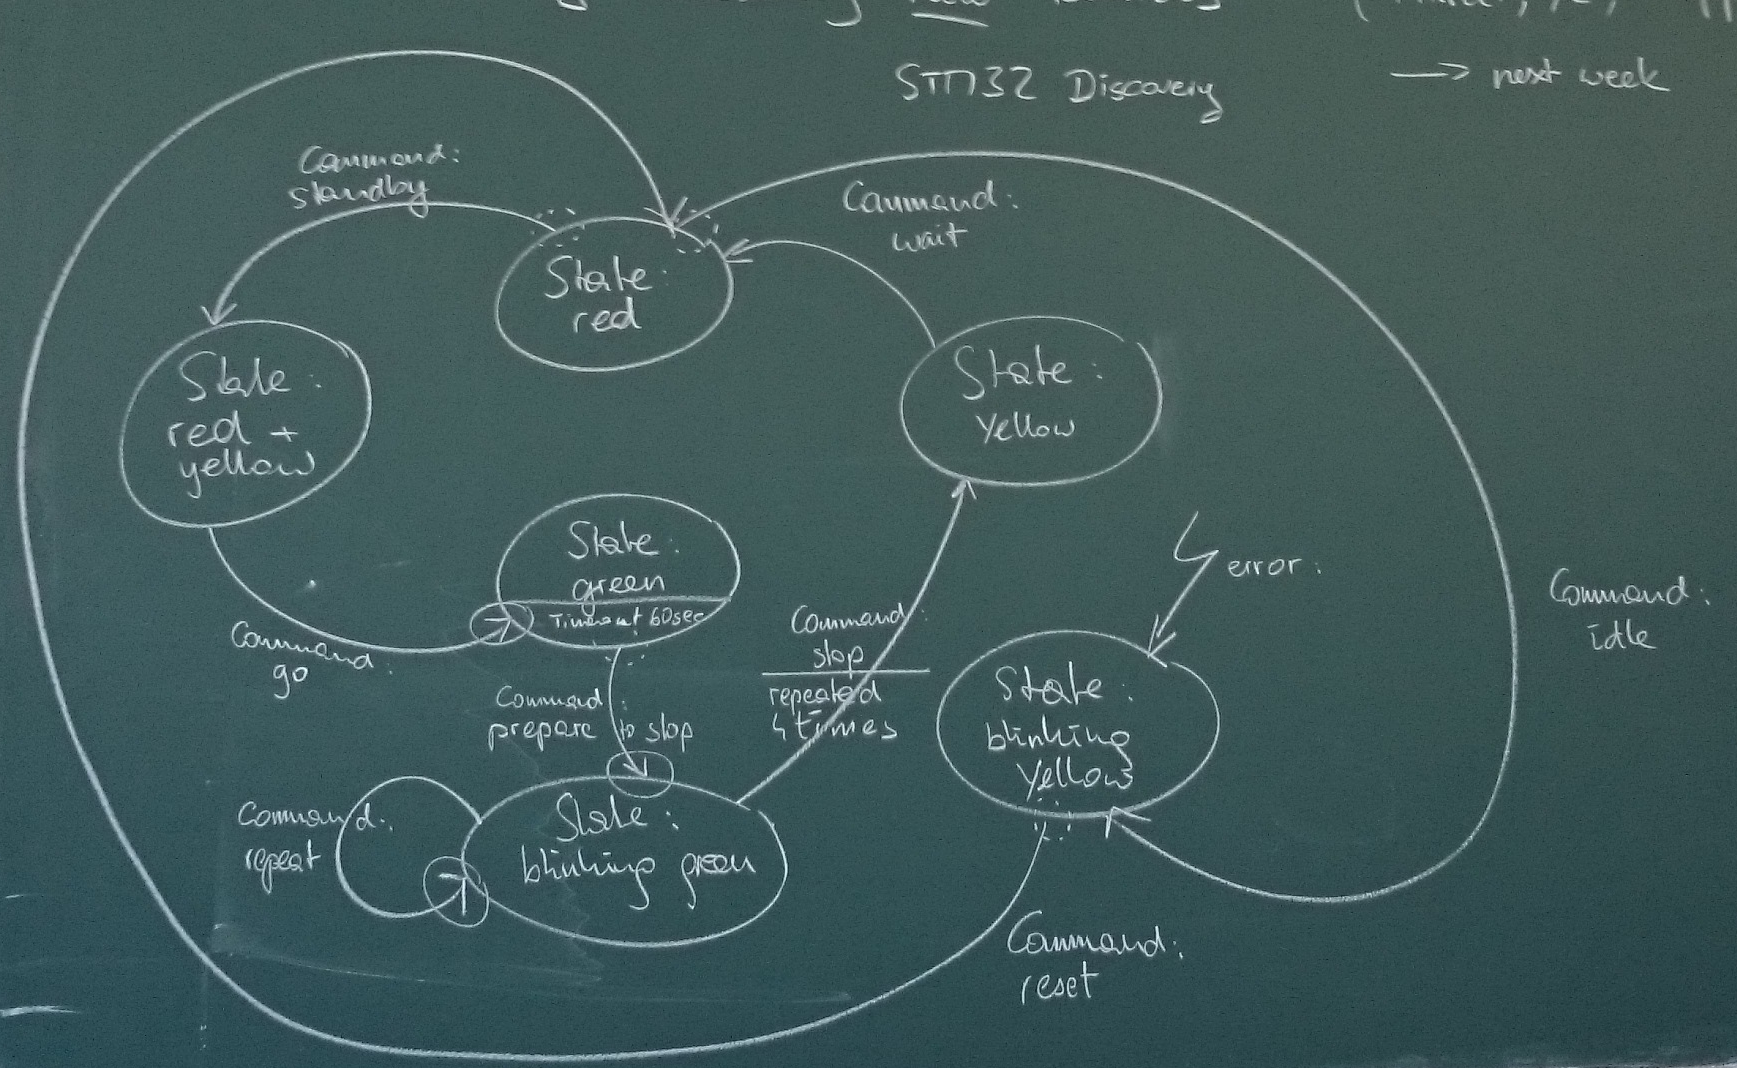
\includegraphics[width=1\linewidth]{angabeTafel.png}
\label{fig:angabeTafel}
\end{figure}

\chapter{Designüberlegung}

Umzusetzen sind folgende 5 State Machine Patterns:
\newline
\begin{enumerate}
	\item StateCentric
	\item StateCentricHidden
	\item EventCentric
	\item StatePattern
	\item TableDriven
\end{enumerate}

\chapter{Aufwandschätzung}

\chapter{Installation \& Durchführung}



\end{document}